\documentclass{amsart}

\usepackage{amsmath, graphicx}

\title{Supplementary Figures for An ``opinion reproduction number'' for infodemics in a bounded-confidence content-spreading process on networks}
\author{Heather Z. Brooks and Mason A. Porter}

\begin{document}
\maketitle

\begin{figure}
    \centering
    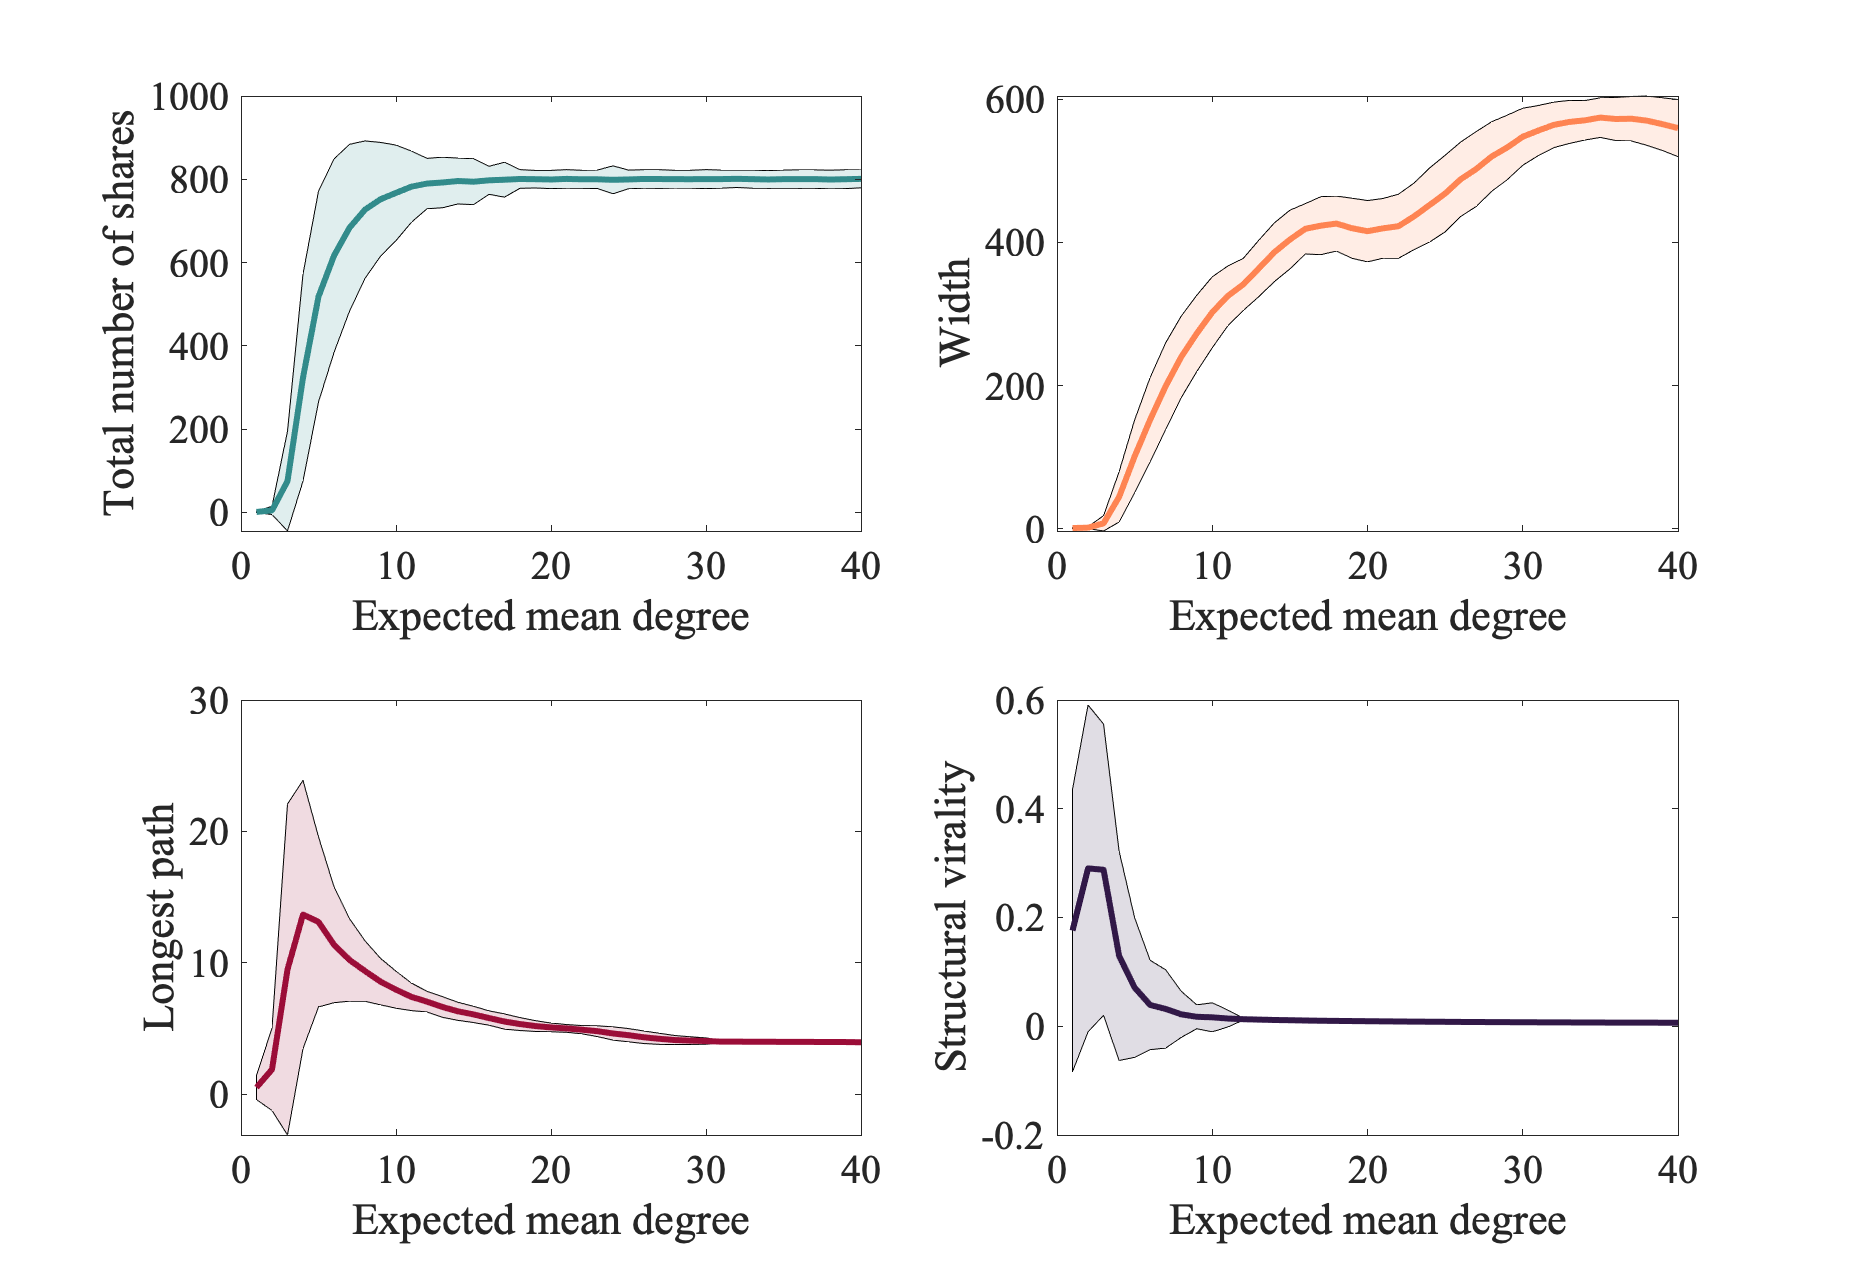
\includegraphics[width=0.9\textwidth]{vary-lambda-compare-x2.png}
    \caption{The effect of varying the expected mean degree $\lambda$ of a network on the total number of content shares, the width, the longest-path length, and the structural virality of dissemination trees of our content-spreading model on configuration-model networks when the opinion value is $x_0=0.2$. 
    We do not see qualitative differences in this figure when $x_0$ is changed; compare to Figure 6 in the manuscript where $x=0.5$. 
    The solid curves give means across $1000$ realizations, and the shaded regions give the standard deviations. In each realization, we generate a 2000-node configuration-model network with a degree sequence from a Poisson distribution with mean $\lambda$. 
    We vary $\lambda$ from $1$ to $40$ in increments of $1$. Each realization has different initial node opinions, which we draw uniformly at random from $(0,1)$. 
    The receptiveness parameter is $c = 0.2$. 
    In each realization, we draw a new degree sequence and a new set of node opinions.}
\end{figure}

\newpage

\begin{figure}
    \centering
    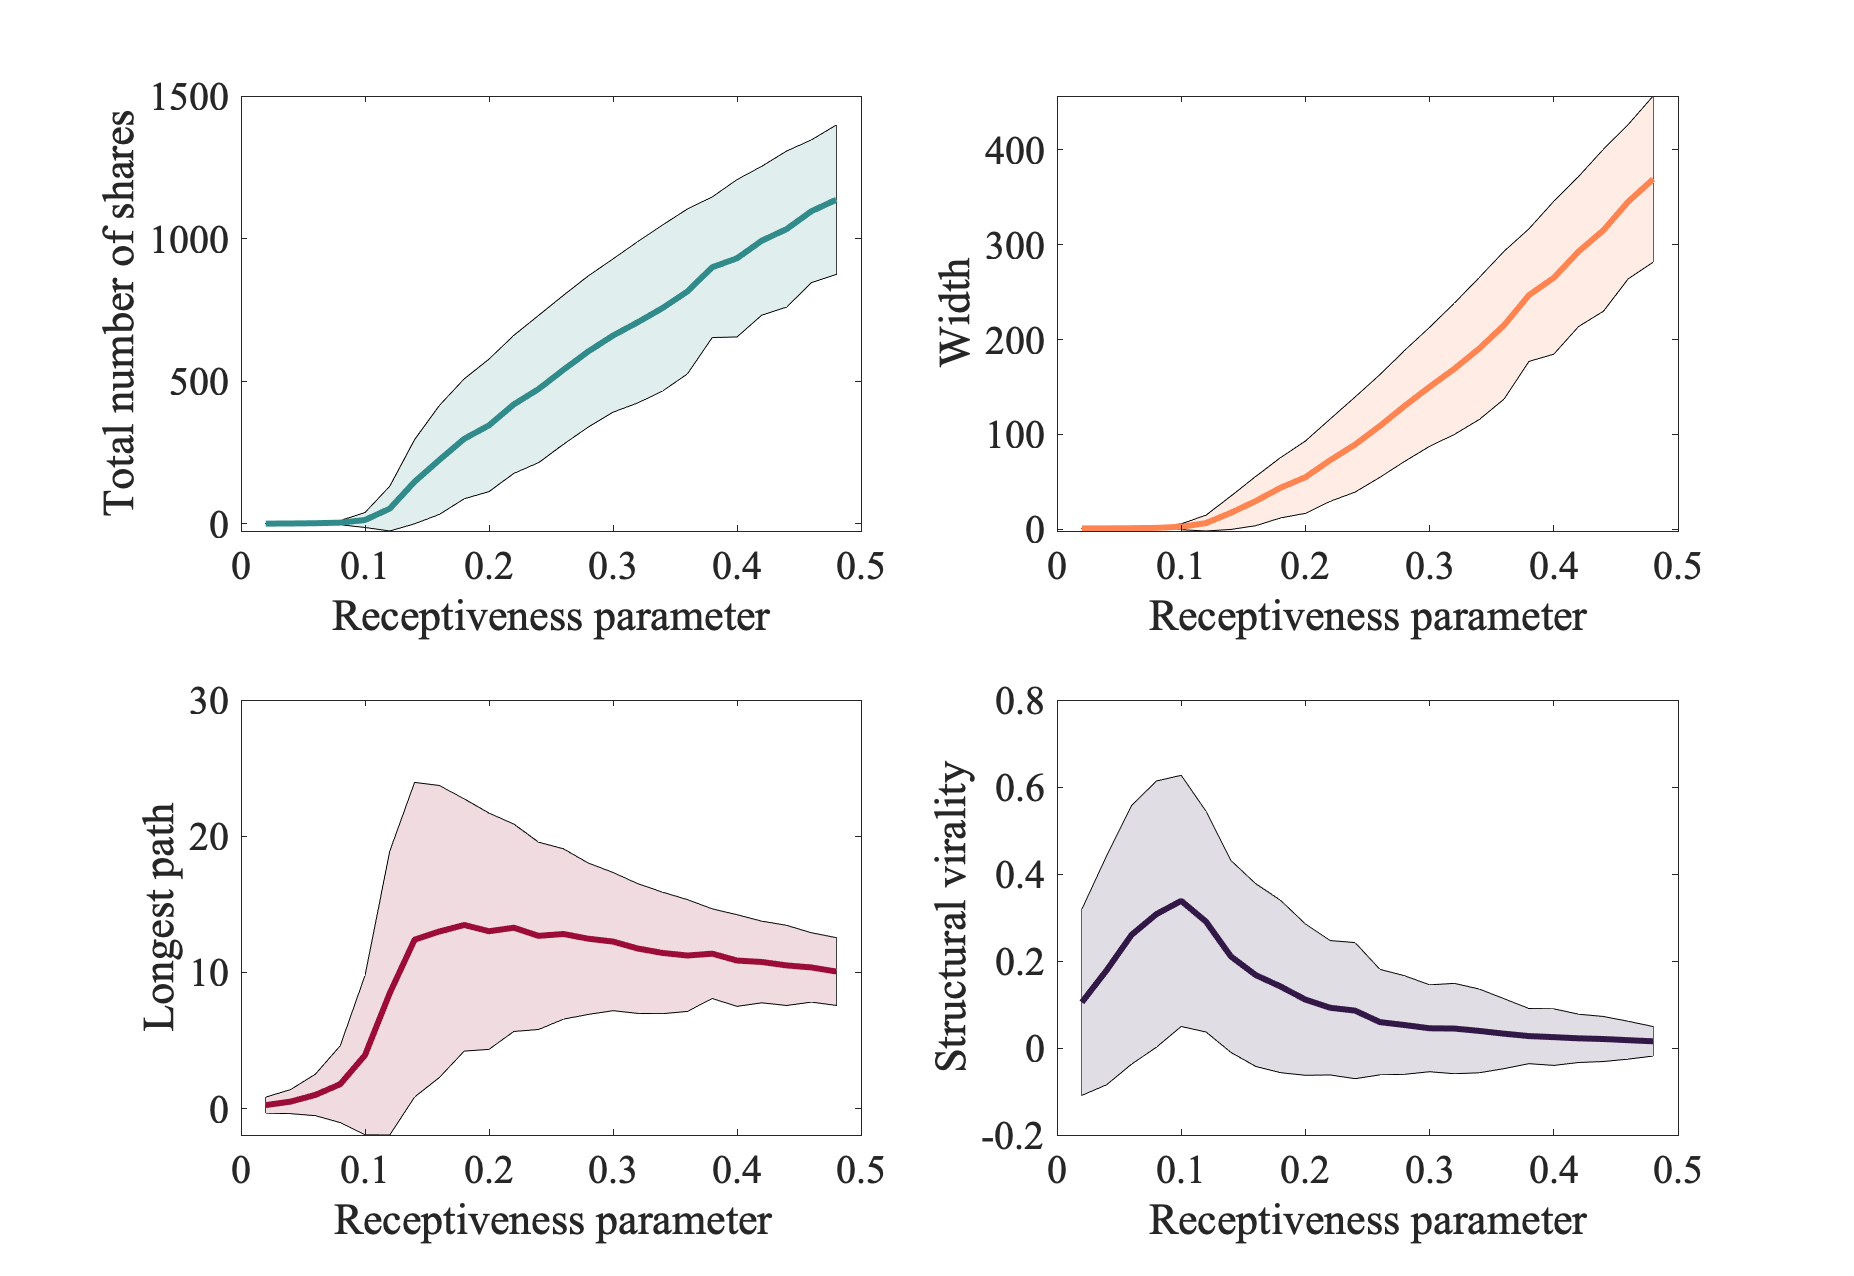
\includegraphics[width=0.9\textwidth]{vary-c-compare-x15.png}
    \caption{The effect of varying the receptiveness parameter $c$ on the total number of content shares, the width, the longest-path length, and the structural virality of dissemination trees of our content-spreading model on configuration-model networks when the opinion value is $x_0=0.15$. We do not see qualitative differences in this figure when $x_0$ is changed; compare to Figure 7 in the manuscript where $x=0.5$.  
    The solid curves give means across $1000$ realizations, and the shaded regions give the standard deviations. In each realization, we generate a 2000-node configuration model network with a degree sequence from a Poisson distribution with mean $\lambda = 5$.
    Each realization has different initial node opinions, which we draw uniformly at random from $(0,1)$. 
    We vary $c$ from $0.02$ to $0.48$ in increments of $0.02$.
    In each realization, we draw a new degree sequence and a new set of node opinions.
    }
\end{figure}

\end{document}